
\mysection[black]{1. Computer Vision}



\mysubsection{1.1 Digital images \& sensors}
An image (as 2D signal) is a continuous function. A pixel is a discrete sample of that cont. function. $I:\{1, \ldots, X\} \times\{1, \ldots, Y\} \rightarrow S$

Some challenges with images: transmission interference, compression artifacts, spilling, scratches, sensor noise, low contrast or resolution, motion blur.

\BDEF{Charge coupled device (CCD)}{  An array of photosites (a bucket of electrical charge) hold charge proportional to incident light intensity during exposure. Charges move down through sensor array, ADC (analog-digital-converter) measures line-by-line.
\begin{enumerate}[leftmargin = *,noitemsep]
\item \textbf{Blooming}: Oversaturated photosites cause vertical channels to "flood" (bright vertical line)
 \item \textbf{Bleeding/Smearing}: While charge in transit, bright light hits photosites above - worse with shorter shutter times (electrical shutters only)
 \item \textbf{Dark current}: CCDs produce thermally generated charge: random noise despite darkness. Avoid by cooling, worsens with age.
 \end{enumerate}
 
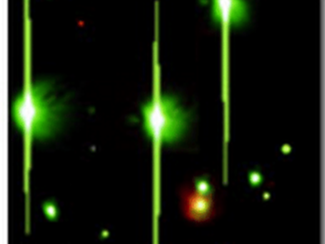
\includegraphics[width=0.32\linewidth]{../images/blooming.png}
 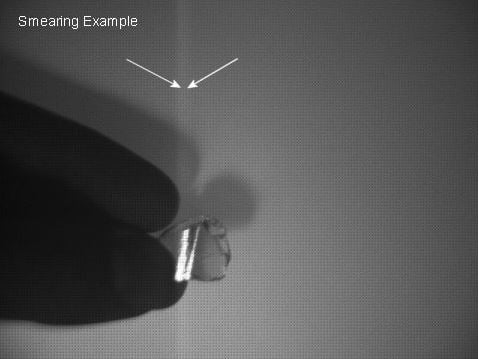
\includegraphics[width=0.32\linewidth]{../images/bleeding.jpg}
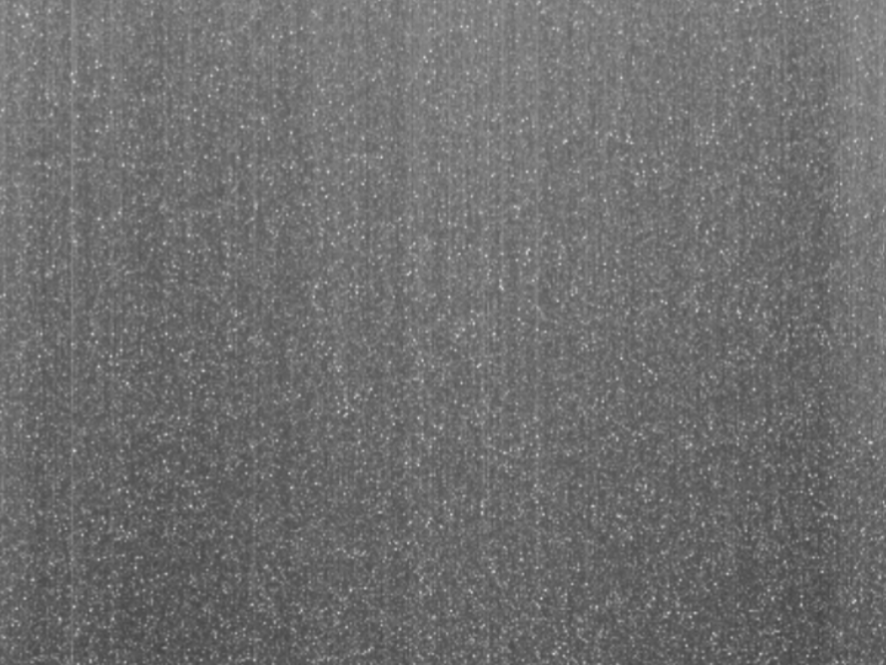
\includegraphics[width=0.32\linewidth]{../images/dark_current.png}


\hspace{0.11\linewidth} (1) \hspace{0.25\linewidth} (2)  \hspace{0.25\linewidth} (3)
}

\BDEF{CMOS Sensors}{  Mostly same as CCD, but each sensor has amplifier. Cheaper, lower power, no blooming, on-chip integration with other components, but less sensitive and more noise. \textbf{Rolling shutter} is an issue for sequential read-out of lines when camera moving. $\Rightarrow$ misalignment/distortions, \textbf{Dark current}}

\textbf{Quantization}: Discretizes measured values into integers. Intrinsically lossy. \\

\textbf{Sampling (spg)}: Measures values at (non-uniform) intervals. Reconstruction possible for uniform spg according to spg theorem otherwise apply low-pass filter \\

\textbf{Undersampling}: Causes loss of information and introduces \textbf{aliasing }(incorrect reconstruction, due to low sampling-rate ).\\

\textbf{Reconstruction}: Sample $\mapsto$ cont. Signal. Needs assumption of behaviour.



\begin{multicols}{2}
\textbf{Bilinear Interpolation}: 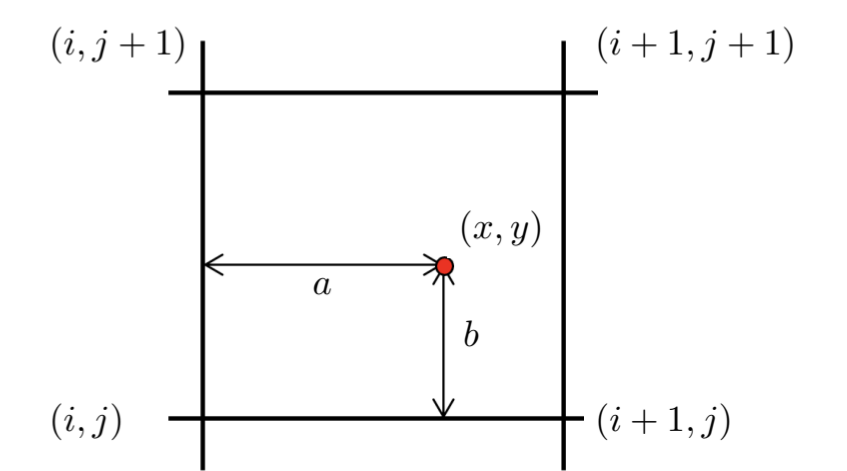
\includegraphics[width=\linewidth]{../images/bilinear.png} 
\columnbreak

Reconstruction ($\hat{f}$) for 2D sampling. Assumes linear behaviour. $ \hat{f}(x, y)=(1-a)(1-b) \cdot f(i, j)\\ + a(1-b) \cdot f(i+1, j) \\ + a b \cdot f(i+1, j+1) \\ +(1-a) b \cdot f(i, j+1)$
\end{multicols}






\BRE{Nyquist-Shannon Sampling Theorem}{Sample freq. ($\omega_s$),highest freq. ($\omega_{max}$): $\omega_s \geq 2 \omega_{max}$ \textbf{Proof}: $h\circ g, h=$ w. $\omega_{max}$, $g=$ grid with spaces $\frac{1}{\omega} \overset{\underset{\mathrm{CT}}{}}{\rightarrow} H\in[-\omega_{max},\omega_{max}]$, $G=$ GwS $\omega$, $H*G\Rightarrow ...$ 

} 


\textbf{Geometric resolution}: \# pixels per area\\
\textbf{Radiometric resolution}: \# bits per pixel\\
\textbf{Image noise}:

\textbf{Additive Gaussian}: $I(x, y)=f(x, y)+c$ where $c \sim$ $N\left(0, \sigma^2\right)$ (so density $\left.p(c)=\left(2 \pi \sigma^2\right)^{-1} e^{\frac{-c^2}{2} \sigma^2}\right)$\\
 \textbf{Poisson (shot) noise}: $p(k)=\frac{\lambda^k e^{-\lambda}}{k!}$.\\ 
 \textbf{Rician noise (MRI)}: $p(I)=$ $\frac{1}{\sigma^2} \exp \left(\frac{-\left(I^2+f^2\right)}{2 \sigma^2}\right) I_0\left(\frac{I f}{\sigma^2}\right)$\\ 
 \textbf{Multiplicative noise}: $I=f+$ $f c$. \\
  \textbf{Signal to noise ratio (SNR)}: Index of image quality: $s=\frac{F}{\sigma}$ where $F=\frac{1}{X Y} \sum_{x=1}^X \sum_{y=1}^Y f(x, y)$.\\
 \textbf{Peak SNR (PSNR)}:$s_{\text {peak }}=\frac{F_{\max }}{\sigma}$.

\textbf{Color camera concepts}: Prism (splitting light, 3 sensors, requires good alignment), Filter mosaic (coat filter on sensor, grid, introduces aliasing), Filter wheel (rotate filter in front of lens, static image), CMOS sensor (absorbing colors at different depths)

\mysubsection{1.2 Image Segmentation}
Partition image into regions of interest. e.g. foreground/background, motion segmentation, ... \\ 
\textbf{Complete segmentation of $I$ }: regions $R_1, \ldots, R_N$ s.t. $I=\bigcup_{i=1}^N R_i$ and $R_i \cap R_j=\emptyset$ for $i \neq j$. \\
\textbf{Chromakeying}: Choose background (BG) color distinct from object (e.g. blue/green vs skin) $\boldsymbol{c}$, then segmentation using BG subtraction with $I_{BG} = \boldsymbol{c}$, Issues: hard $\alpha$-mask, variation not same in 3 channels
\BCODE{Thresholding}{Produces binary image by labeling pixels \textit{in} or \textit{out} by comparing to some threshold $T$ (RGB: $T \in  \mathbb{R}^3$, Gray:  $T \in  \mathbb{R}$)
$B(x, y) = 1 $ if $ \mathbf{I}_{\alpha}(x, y) >= T $ else $0$, finding $T$ with trial and error, compare results with ground truth. Result: $\mathbf{I}_{\text {proc}}=\mathbf{I}_\alpha \cdot \mathbf{I}+\left(1-\mathbf{I}_\alpha\right) \cdot \mathbf{I}_{BG}$  
}
\textbf{Distance Measures} $\mathbf{I}_{\alpha}$
\begin{itemize}[leftmargin= *]
\item \textbf{BG Subtraction}: $\mathbf{I}_\alpha=\left|\mathbf{I}-\mathbf{I}_{\mathrm{BG}}\right|$
\item \textbf{Mahalanobis}:  $\mathbf{I}}_\alpha=\sqrt{\left(\mathbf{I}-\mathbf{I}_{\mathrm{BG}}\right)^T \Sigma^{-1}\left(\mathbf{I}-\mathbf{I}}_{\mathrm{bg}}\right)}$ where $\Sigma$ is the BG image's covariance matrix: $\Sigma_{i j}=\mathbb{E}\left[\left(X_i-\mu_i\right)\left(X_j-\mu_j\right)\right]$, estimate it from $n \geq 3$  data points. to guarantee invert. of $\Sigma$, need $3$ ind. samples : $\frac{1}{n-1} \sum_{i=1}^n\left(x_i-\mu\right)\left(x_i-\mu\right)^T$,$\mu:=\frac{1}{n}\Sigma_{i=1}^nx_i$

\end{itemize}


\BCODE{Receiver operating characteristic (ROC)}{
Describes performance of binary classifier (x: FPR y: TPR). With (table same as integral)
\begin{itemize}[leftmargin = *,noitemsep]
\item true pos. (\textcolor{matplotlibgreen}{\textbf{TP}}): $\#$ corr. classified FG, $\int_{\tau}^{\infty}f_{\operatorname{p}}dx$
\item false pos. (\textcolor{matplotlibred}{\textbf{FP}}): $\#$ BG wrongly clas. as FG, $\int_{\tau}^{\infty}f_{\operatorname{n}}$
\item false neg. (\textcolor{matplotlibgreen}{\textbf{FN}}): $\#$ FG wrongly clas. as BG, $\int_{0}^{\tau}f_{\operatorname{p}}$
\item true neg. (\textcolor{matplotlibred}{\textbf{TN}}): $\#$ corr. clas. BG, $\int_{0}^{\tau}f_{\operatorname{n}}dx$

\item true pos. rate (\textbf{TPR}) : $\frac{T P}{T P+F N}=1-$\textbf{FNR}
\item false pos. rate (\textbf{FPR}) : $\frac{FP}{F P+T N}=1-$\textbf{TNR}
\end{itemize}


\textbf{Trade-Off-Metric}: 
$\beta=\frac{T N+F P}{T P+F N} \cdot \frac{V_{\mathrm{TN}}+C_{\mathrm{FP}}}{V_{\mathrm{TP}}+C_{\mathrm{FN}}}$, $V$: Val. corr. clas., $C$: Cost for misclassifications\\ \textbf{Naming}: TPR=sensitivity, FPR=1-specificity, FNR = $\frac{FN}{T P+F N}$, TNR = $\frac{TN}{F P+T N}$, Prec = $\frac{TP}{T P+ FP	}$  
}
\begin{center}
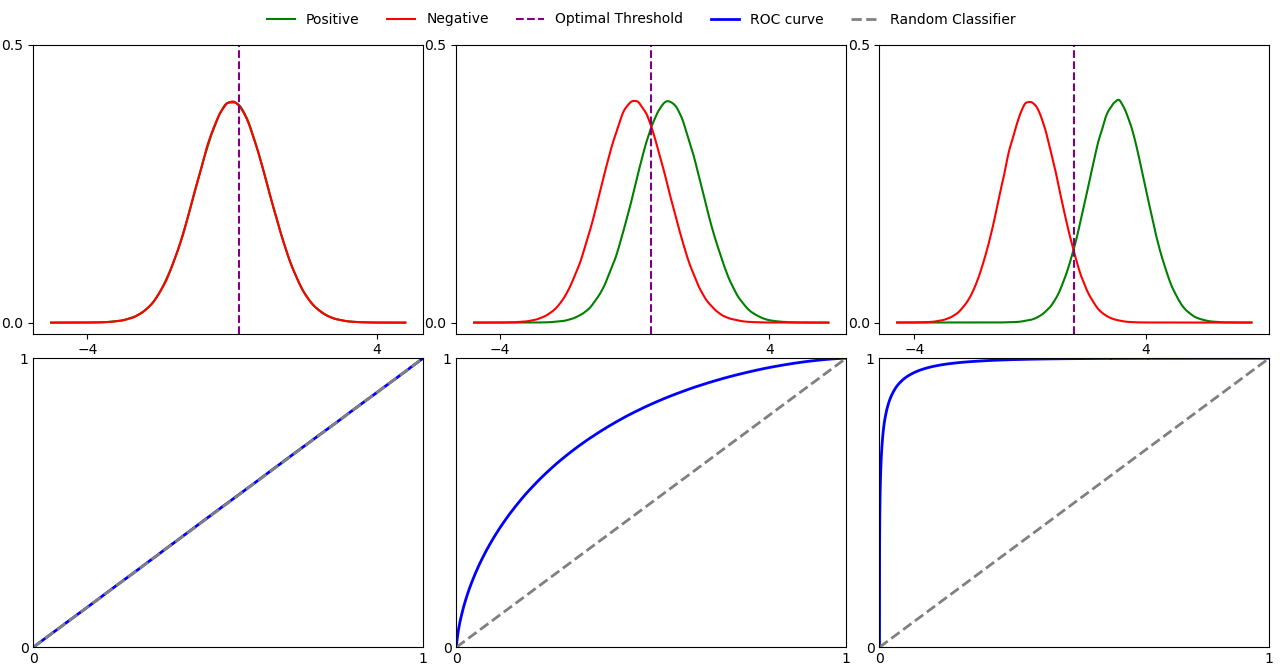
\includegraphics[width=\linewidth]{../images/ROC.png} 
\end{center}


\textbf{Pixel neighbourhoods}: 4/8-connectivity: 4-neighb. means horiz. + vert. or 8-neighb. with diag.\\

\textbf{Connected Component Labelling (CCL)}: Image processing technique to identify connected pixel regions.


\BCODE{Region Growing}{
\begin{enumerate}[leftmargin = *,noitemsep]
\item Select initial region/seed (manually or conservative thresholding)
\item Add neighbouring pixels if criteria satisfied
\item Repeat until no pixels can be added
\end{enumerate}
}
\textbf{Criterias} %ROUT
\begin{itemize}[leftmargin = *,noitemsep]
\item \textbf{Grey-Level-Thresholding}: Apply simple thresholding
\item \textbf{Advanced}: Compute std-deviation $\sigma$, mean $\mu$ of graylevels in region and check $\left.(I(x, y)-\mu)^2<(n \sigma)^2\right)$

\end{itemize}

\BCODE{Snakes}{Active contour, polygon, where each point on contour moves away from seed while inclusion criteria in neighborhood is met, often smoothness constraint. Iteratively minimize energy: $E=E_{\text {tension }}+E_{\text {stiffness }}+$ $E_{\text {image }}$}
\textbf{Markov Random fields}: Cost to assign label to each pixel, cost to assign pair of labels to connected pixels. Solve with graph cuts, source $=$ FG, sink $=$ BG. Minimize energy in polynomial time using MinCut. To get decent results, we need alpha estimation / border matting along edges. \\


\BDEF{Morphological Operations}{
Op that applies structuring element $S$ to the neighborhood of each pixel in $I$. Sets with x-y-coords. of $1$s. 
\begin{itemize}[leftmargin = *,noitemsep]
 
\item \textbf{Dilation of $I$}: $D=I \oplus S$, apply $D(p)$ to all pixels
\item \textbf{Erosion of $I$}: $E=I \ominus S$, apply $E(p)$ to all pixels
\item \textbf{Hit-and-Miss}: $H=I \otimes S$ exact match of $I$ by $S$
\item \textbf{Opening}: $O = I \circ S=(I \ominus S) \oplus S$
\item \textbf{Closing}:  $C = I \bullet S=(I \oplus S) \ominus S$

\item \textbf{Thinning}: $I \oslash S=I \backslash(I \otimes S)$
\item \textbf{Tickening}: $ I \odot S=I \cup(I \otimes S)$
\end{itemize}

}
\textbf{Definitions}:
\begin{itemize}[leftmargin = *,noitemsep]
\item $S$ \textbf{fits} $I$ at $p$ if $\{y: y=p+s, s \in S\} \subset I$
\item $S$ \textbf{hits} $I$ at $p$ if $\{y: y=p-s, s \in S\} \cap I \neq \emptyset$
\item $S$ \textbf{misses} $I$ at $p$ if: $\{y: y=p-s, s \in S\} \cap I=\emptyset$

\item \textbf{Dilation at $p$}: $D(p)= 1 \text { if } S \text { hits } I \text { at } p  \text { else } 0$
\item \textbf{Erosion at $p$}: $E(p)=1 \text { if } S \text { fits } I \text { at } p \text { else } 0$\


\end{itemize}

\begin{center}
 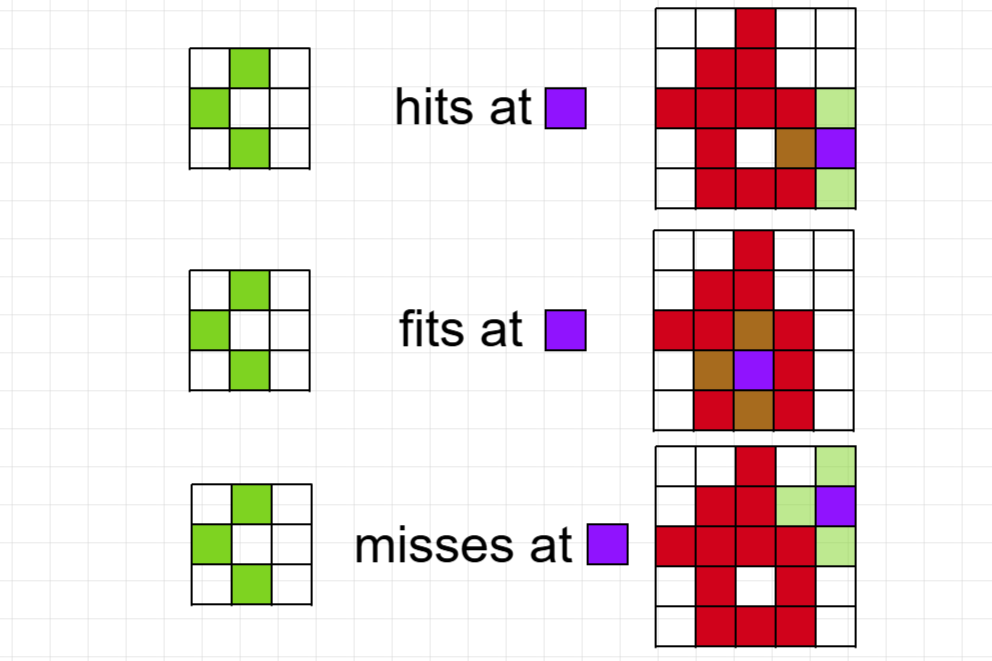
\includegraphics[width=0.48\linewidth]{../images/OP2.png}
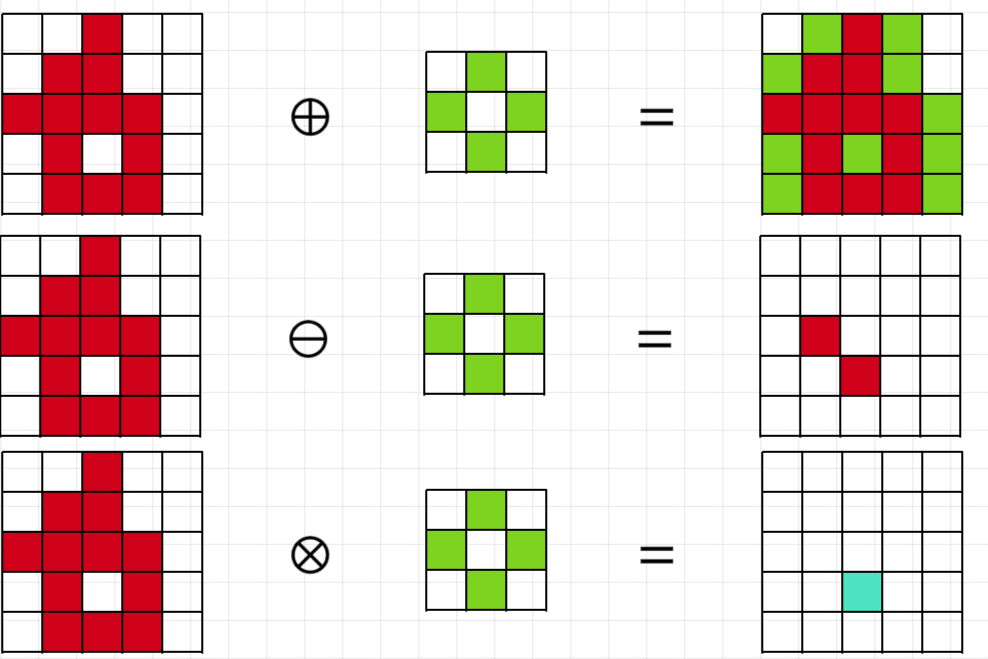
\includegraphics[width=0.48\linewidth]{../images/OP.png}

\end{center}

It holds that: $(I \odot S)^{\complement}=I^{\complement} \oslash S$

\BDEF{Skeleton and Medial Axis Tansform (MAT) }{Stick figure representations of region $X \subset \mathbb{R}^2$.
Skeleton: union of centres of max. discs within $X$.

$
B=\{(2,1),(2,1),(2,2),(2,3),(3,2)\} \hat{=}\left(\begin{array}{lll}
0 & 1 & 0 \\
1 & 1 & 1 \\
0 & 1 & 0
\end{array}\right)
$

$S_{n(X)}=\left(X \ominus_n B\right) \backslash\left(\left(X \ominus_n B\right) \circ B\right)$ is the $n$-th skeleton subset. Skeleton is: $S(x)=\bigcup_{n=1}^{\infty} S_n(x)$ Reconstr.: $X=\bigcup_{n=0}^{\infty} S_{n(X)} \oplus_n B$ Used in object / char. recogn. Sensitive to noise, def. on digital grid poorly defined. Seq. thin. sometimes referred.


}



\mysubsection{1.3 Image Filtering}

\textbf{Shift-invariant}: same for all pixels, $K$ not dep. on $x,y$\\
\textbf{Linear}: Lin. comb. of nhb. $\alpha L\left(I_1\right)+\beta L\left(I_2\right)=$ $L\left(\alpha I_1+\beta I_2\right)$  Mult. with $I(x,y)\Rightarrow \text{lin}$. Can be written $K(i, j)=a i+b j+c$. If $2^{K(i,j)}$ is separable.  \\
\textbf{Shift}: $K=(\begin{smallmatrix}
0 & 0 & 0 \\ 
0 & 0 & 1 \\ 
0 & 0 & 0
\end{smallmatrix})\Rightarrow$ conv. shifts to right, shift invariant

\BDEF{Correlation $K \circ I$}{
$I^{\prime}(x, y)=\sum_{(i, j) \in N(x, y)} K(i, j) I(x+i, y+j)$
}

\BDEF{Convolution $K * I$}{
$
I^{\prime}(x, y)= \sum_{(i, j) \in N(x, y)} K(i, j) I(x-i, y-j)
$


Lin., ass., shift-invariant, comm. (if dims are same). For cont.: $g(x)=$ $f(x) * k(x)=\int_{\mathbb{R}} f(\tau) k(x-\tau) \mathrm{d} \tau$}

$K * I = K^{\prime} \circ I$ where: $K(i, j)=K'(-i,-j)$ 

\textbf{Padding}: clip to black, wrap around, copy edge, reflect across edge, vary filter!\\
\textbf{Separable}: $K(m, n)\in \mathbb{R}^{m\times m}=f(m) g(n)$ more eff. apply first $f\in \mathbb{R}^{m\times 1}$, then $g\in \mathbb{R}^{1\times m}$ on image$\in \mathbb{R}^{h\times w}$ $\mathcal{O}(w\cdot h \cdot m^2) \mapsto \mathcal{O}(w\cdot h \cdot m)$\\
\textbf{Gaussian}: $ G_\sigma= \frac{1}{2 \pi \sigma^2} e^{-\frac{x^2+y^2}{2 \sigma^2}}$, rot. symmetric, single lobe, FT is again a Gaussian, separable, easily made efficient. Used to smooth, reduce noise, padding w. 0 or clamping. \textbf{Prove low-pass} $\mathcal{F}(G_\sigma)\circ \mathcal{F}(I) \overset{\underset{\mathrm{CT}}{}}{=} G_\sigma\circ \mathcal{F}(I)$ High freq. mult. with small number, \textbf{Idea} weigh by dist.


\BEX{Kernel Examples $K_x = K_y^{T}$}{
\begin{tabular}{lllll}
Low-pass &  High-pass &  Laplacian &  Prewitt(x)\\
$\frac{1}{9}
\left(
\begin{smallmatrix}
1 & 1 & 1 \\ 
1 & 1 & 1 \\ 
1 & 1 & 1
\end{smallmatrix}
\right)$ &
$\left(
\begin{smallmatrix}
-1 & -1 & -1 \\ 
-1 & 8 & -1 \\ 
-1 & -1 & -1
\end{smallmatrix}
\right) $ &

$ \left(
\begin{smallmatrix}
0 & 1 & 0 \\ 
1 & -4 & 1 \\ 
0 & 1 & 0
\end{smallmatrix}
\right)$ &

$\left(
\begin{smallmatrix}
-1 & 0 & 1 \\ 
-1 & 0 & 1 \\ 
-1 & 0 & 1
\end{smallmatrix}
\right) $ \\
 Sobel(x) & Id  & F-Diff.(x) & C-Diff.(x)  \\

$\left(
\begin{smallmatrix}
1 & 0 & -1 \\ 
-2 & 0 & 2 \\ 
-1 & 0 & 1
\end{smallmatrix}
\right) $ & 
$\left(
\begin{smallmatrix}
0 & 0 & 0 \\ 
0 & 1 & 0 \\ 
0 & 0 & 0
\end{smallmatrix}
\right) $
&

$\left(
\begin{smallmatrix}
-1 & 1 
\end{smallmatrix}
\right)$
&
$\left(
\begin{smallmatrix}
-1 & 0 & 1 
\end{smallmatrix}
\right)$

\end{tabular}
}

\textbf{Image sharpening}: enhances edges by increasing high frequency components: $I^{\prime}=I+\alpha|k * I|$ where $k$ highpass filter, $\alpha \in[0,1]$.\\

\textbf{Partial Derivatives}: Can be approximated if $I$ is discrete by convolution with different Kernels.
$
\frac{\partial f}{\partial x}=\lim _{\varepsilon \rightarrow 0}\left(\frac{f(x+\varepsilon, y)}{\varepsilon}-\frac{f(x, y)}{\varepsilon}\right) \approx \frac{f\left(x_{n+1}, y\right)-f\left(x_n, y\right)}{\Delta x}
$
Larger = Better due: nghb affected by freq noise. $\Rightarrow$ mix deriv. filter with low pass by extending filter
\begin{itemize}[leftmargin = *,noitemsep]
\item \textbf{Laplacian}: Edges all dir, $\nabla ^2$-appr. noise-sensitive, requires pre-smoothing. Zero-crossing for edge det.
\item \textbf{Prewitt}: Edges in x,y-dir. More sensitive to noise than Sobel.
\item \textbf{Sobel}: Smooths via central weights, better edge det than Prewitt. May require thresholding
\item \textbf{F-Diff}:  Compute first-order derivatives; $\nabla$-appr.
\item \textbf{C-Diff}: More accurate than forward diff.
\end{itemize}

Here: $\nabla^2 f(x, y)=\frac{\partial^2 f(x, y)}{\partial x^2}+\frac{\partial^2 f(x, y)}{\partial y^2}$


\mysubsection{1.4 Edge Detection}

\BDEF{Laplacian operator}{Find 0 s in 2nd deriv $I^{\prime \prime}$ to locate edges. Rot. invariant, yields very noisy but thin and uninterrupted edges. Sensitive, blur first (Laplacian of Gaussian) or suppress edges with low gradient magnitude.}


\BDEF{Laplacian of Gaussian (LoG)}{
Blurring of image with Gaussian and Laplacian operator can be combined into convolution with LoG:
$$\operatorname{LoG}(x, y)=-\frac{1}{\pi \sigma^4}\left(1-\frac{x^2+y^2}{2 \sigma^2}\right) \exp \left(-\frac{x^2+y^2}{2 \sigma^2}\right)$$
}




\BCODE{Canny Edge Detector }{Thin, interrupted edges, extended more completely than with simple thresh.
\begin{enumerate}[leftmargin =*]
\item \textbf{Smoothing image}: with Gaussian filter
\item \textbf{Compute gradient, magnitude \& orientation} :  Use Sobel, Prewitt, ...
$
M(x, y)=\sqrt{\left(\frac{\partial f}{\partial x}\right)^2+\left(\frac{\partial f}{\partial y}\right)^2}, \alpha(x, y)=\tan ^{-1}\left(\frac{\partial f}{\partial y} / \frac{\partial f}{\partial x}\right)
$
\item \textbf{Nonmaxima suppression}: quantize edges normal to 4 dirs, if smaller than either neighb. suppress
\item \textbf{Double thresholding}: Classify pixels as \textit{strong-} , \textit{weak-} or \textit{non-edges}: $E_{strong}\geq \theta_{high}> E_{weak}\geq \theta_{low}$
\item \textbf{Edge Tracking (Hysteresis)}: Classify $E_{weak}$ that are not 8-conn. to $E_{strong}$ as \textit{non-edge}.
\end{enumerate}
}

\BCODE{Hough Transformation}{Maps cart. coords. $(x,y)$ to parameter Space (p.S) to detect specific form.
\begin{enumerate}[leftmargin = *,noitemsep]
\item \textbf{Subdivide p.S.}: Into discrete bins init to $0$. 
\item \textbf{Vote in p.s.}: For each edge-pixel in $(x,y)$ compute potential points, map onto p.s.
\item \textbf{Detect peaks in p.s.}: Corresponds to form in $(x,y)$
\end{enumerate}}

\begin{itemize}[leftmargin=*]
\item \textbf{Lines (slope)} : Choose $m\in [a,b]$; compute $c=y-mx$; Plot $(m,c)$; has $\infty$ slope problem.
\item \textbf{Lines (polar)} : Choose $\theta \in [0,\pi]$; Compute $ \rho = x \cos \theta + y \cos \theta$; Plot $(\rho,\theta)$
\item \textbf{Circles}: Choose $\theta \in [0,2\pi],r\in[0,c] $; Compute $a=x-r\cos \theta, b = y-r\sin \theta$; Plot $(a,b,r)$
\item \textbf{Parabola}: Choose $a,b \in \mathbb{R}$; Compute $c=y-ax-bx^2$
\end{itemize}
\textbf{Corner detection}: Properties: acc. local., invar. against shift, rot., scale, brightness, noise robust, repeatability. Corners important since edges only well localized in 1 direction.\\
\textbf{Local Displacement Sensitivity}: Appr. change in intensity $f$ for small shifts $S(\Delta x, \Delta y)=\sum_{(x, y) \in \text { window }}(f(x, y)-f(x+\Delta x, y+\Delta y))^2$. 


Using the linear approx. $f(x+\Delta x, y+\Delta y) \approx$  $f(x, y)+f_x(x, y) \Delta x+f_y(x, y) \Delta y$ we get $S(\Delta x, \Delta y) \approx \sum_{(x, y) \in \text { window }}\left[f_x(x, y) \Delta x+f_y(x, y) \Delta y\right]^2$. We write $S(\Delta x, \Delta y)=(\Delta x \Delta y) \mathbf{M}\binom{\Delta x}{\Delta y} = \Delta^T \mathbf{M} \Delta$ with 
$\mathbf{M}=\sum_{(x, y) \in \text { window }}\left(\begin{array}{cc}f_x^2 & f_x f_y \\ f_x f_y & f_y^2\end{array}\right)$\\

\textbf{Extracting Feature points}: $\lambda_1, \lambda_2$ of $ \mathbf{M}$ we can detect:
\begin{itemize}[leftmargin =*]
\item \textbf{Corner}: $\lambda_1,\lambda_2$ large, same as $\min _{\|\Delta\|=1} \Delta^T \mathbf{M} \Delta$
\item \textbf{Edge}: $\lambda_1 \gg \lambda_2$ or $\lambda_2 \gg \lambda_1$
\item \textbf{Flat Region}: $\lambda_1,\lambda_2$ small
\end{itemize}




\BCODE{Harris Corner Detection}{Avoids EV computation. Uses appr. 
\begin{enumerate}[leftmargin = *,noitemsep]
\item \textbf{Compute} $\mathbf{M}$: 
\item \textbf{Compute} $C$ : $C(x, y)=\operatorname{det}(\mathbf{M})-k \cdot(\operatorname{trace}(\mathbf{M}))^2=\lambda_1 \lambda_2-$ with $k \in [0.04,0.06]$.
\item \textbf{Classify}: corner ($C>0$), edge ($C<0$) or flat region ($|C|$ small) 
\item \textbf{Nonmax suppression}: On corners
\end{enumerate}
Properties:
\begin{itemize}[leftmargin = *,noitemsep]
\item Invariant to shift: $\nabla$ only shifted
\item Inv. to rot: EV stay, eigenvectors rotate
\item Inv. to brightness offset: $\nabla(I+c)=\nabla(I)$
\item not Inv to scaling: $\left(\Delta_z, \Delta_y\right)$ is constant size: corner $>$ wdw-size $\Rightarrow$ edges
\end{itemize}
 }

\BDEF{Lowe's Scale Invariant Feature Transform (SIFT)}{
Used to track feature over multiple images.
\begin{enumerate}[leftmargin = *,noitemsep]
\item \textbf{Create scale space}: Build scale space by using DoG for different $k$.
\item \textbf{Keypoint localization}: Find keypoints, which are extremas by considering neighborhood of current image (8 px), neighborhood of image one scale up and down (9 px each).  
\item \textbf{Orientation assignment}: Compute gradient of neighborhood of keypoints, $m(x, y)= \sqrt{A^2 + B^2}$, $\theta(x, y)=\tan^{-1}(B/A)$ where $A = (L(x+1, y)-L(x-1, y))$ $B=(L(x, y+1)-L(x, y-1))$ and $L$ is the Gaussian-smoothed image at the keypoint's scale. Build histograms with $36$ bins over $360\deg$. Assign peak of the histogram as orientation to the keypoint
\item \textbf{Keypoint descriptor generation}: Take $16\times 16$ neighborhood around keypoint, divide into $4\times 4$ subblocks and compute an 8-bin orientation histogram based on the gradient directions. Results in $128$ feature vector per keypoint.

\end{enumerate}
}

\textbf{Enhance invariance to illumination}: Take resulting feature vector and normalise it. If illumination is non-linear threshold unit vector to 0.2 and then normalise again. \\
\textbf{Difference of Gaussian (DoG)}: Appr. LoG, good in detecting edges, blob-like structures, $D o G(x, y)=\frac{1}{k} e^{-\frac{x^2+y^2}{(k \sigma)^2}}-e^{-\frac{x^2+y^2}{\sigma^2}}$ Same as difference of two Gaussians with scale $\sigma$ and $k\sigma$.

\mysubsection{1.5 Fourier Transform}


\BDEF{Discrete Fourier Transform }{Represents signal in new basis: Transforming from spatial domain $f$ to freq. domain $F$ by: 

$$
F(I)(u, v)=\iint_{R^2} I(x, y) \mathrm{e}^{-i 2 \pi(u x+v y)} d x d y
$$}
\textbf{Inverse}:
$I(x, y)=\iint_{R^2} F(I)(u, v) \mathrm{e}^{i 2 \pi(u x+v y)} d u d v$\\
\textbf{Discrete FT}: $F(u, v)=\sum_{x=0}^{N-1} \sum_{y=0}^{M-1} I(x,y)$  $\cdot e^{-i 2 \pi\left(\frac{u x}{N}+\frac{v y}{M}\right)}$, where $N \times M$ is the image size, $I(x, y)$ the image value at pixel $(x, y)$ and $F(u, v)$ the Fourier coefficient at coordinates $(u, v)$. Can write as $F=\mathbf{U}f$, where $F,f\in \mathbb{C}^{N\cdot M},\mathbf{U}\in \mathbb{C}^{N\cdot M \times N\cdot M}$ dim: in = out\\


\textbf{Def}: $\cos (x)=\frac{e^{i x}+e^{-i x}}{2} \quad \sin (x)=\frac{e^{i x}-e^{-i x}}{2}$ \\ \textbf{Dirac delta}: $\delta(x)=0$ if $x \neq 0$ else undefined with $\int_{-\infty}^{\infty} \delta(x) \mathrm{d} x=1$\\
 
\textbf{Sampling}: Mult with seq. of $\delta$-fnts $F\left(\delta\left(x-x_0\right)\right)(u)=e^{-i 2 \pi u x_0}$. and $\operatorname{sinc}(u)=\frac{\sin (u)}{u}$


\begin{tabular}{lll} 
\textbf{Property }& $\boldsymbol{f}(\boldsymbol{x})$ & $\boldsymbol{F}(\boldsymbol{u})$ \\
Linearity & $\alpha f_1(x)+\beta f_2(x)$ & $\alpha F_1(u)+\beta F_2(u)$ \\
Duality & $F(x)$ & $f(-u)$ \\
Convolut. & $(f * g)(x)$ & $F(u) \circ G(u)$ \\
Product & $f(x) g(x)$ & $(F * G)(u)$ \\
Timeshift & $f\left(x-x_0\right)$ & $e^{-2 \pi i u x_0} \cdot F(u)$ \\
Freq. shift & $e^{2 \pi i u_0 x} f(x)$ & $F\left(u-u_0\right)$ \\
Different. & $\frac{\mathrm{d} n}{\mathrm{~d} x^n} f(x)$ & $\left(\frac{i}{2 \pi} u\right)^n F(u)$ \\
Multiplic. & $x f(x)$ & $\frac{i}{2 \pi} \frac{\mathrm{~d}}{\mathrm{~d} u} F(u)$
\end{tabular}

\textbf{Element-Wise Multiplication}: $\circ$
\BCODE{Image Restoration}{Image degradation is applying kernel $h$ to some image $f$. The inverse $\tilde{h}$ should compensate: $f(x) \rightarrow h(x) \rightarrow g(x) \rightarrow \tilde{h}(x) \rightarrow f$. Determine with $F(\tilde{h})(u, v)=F(h)(u, v)=1$. Cancellation of freq., noise amplif. Regularize using $\tilde{F}(\tilde{h})(u, v)=$ $F(h) /\left(|F(h)|^2+\varepsilon\right)$
}
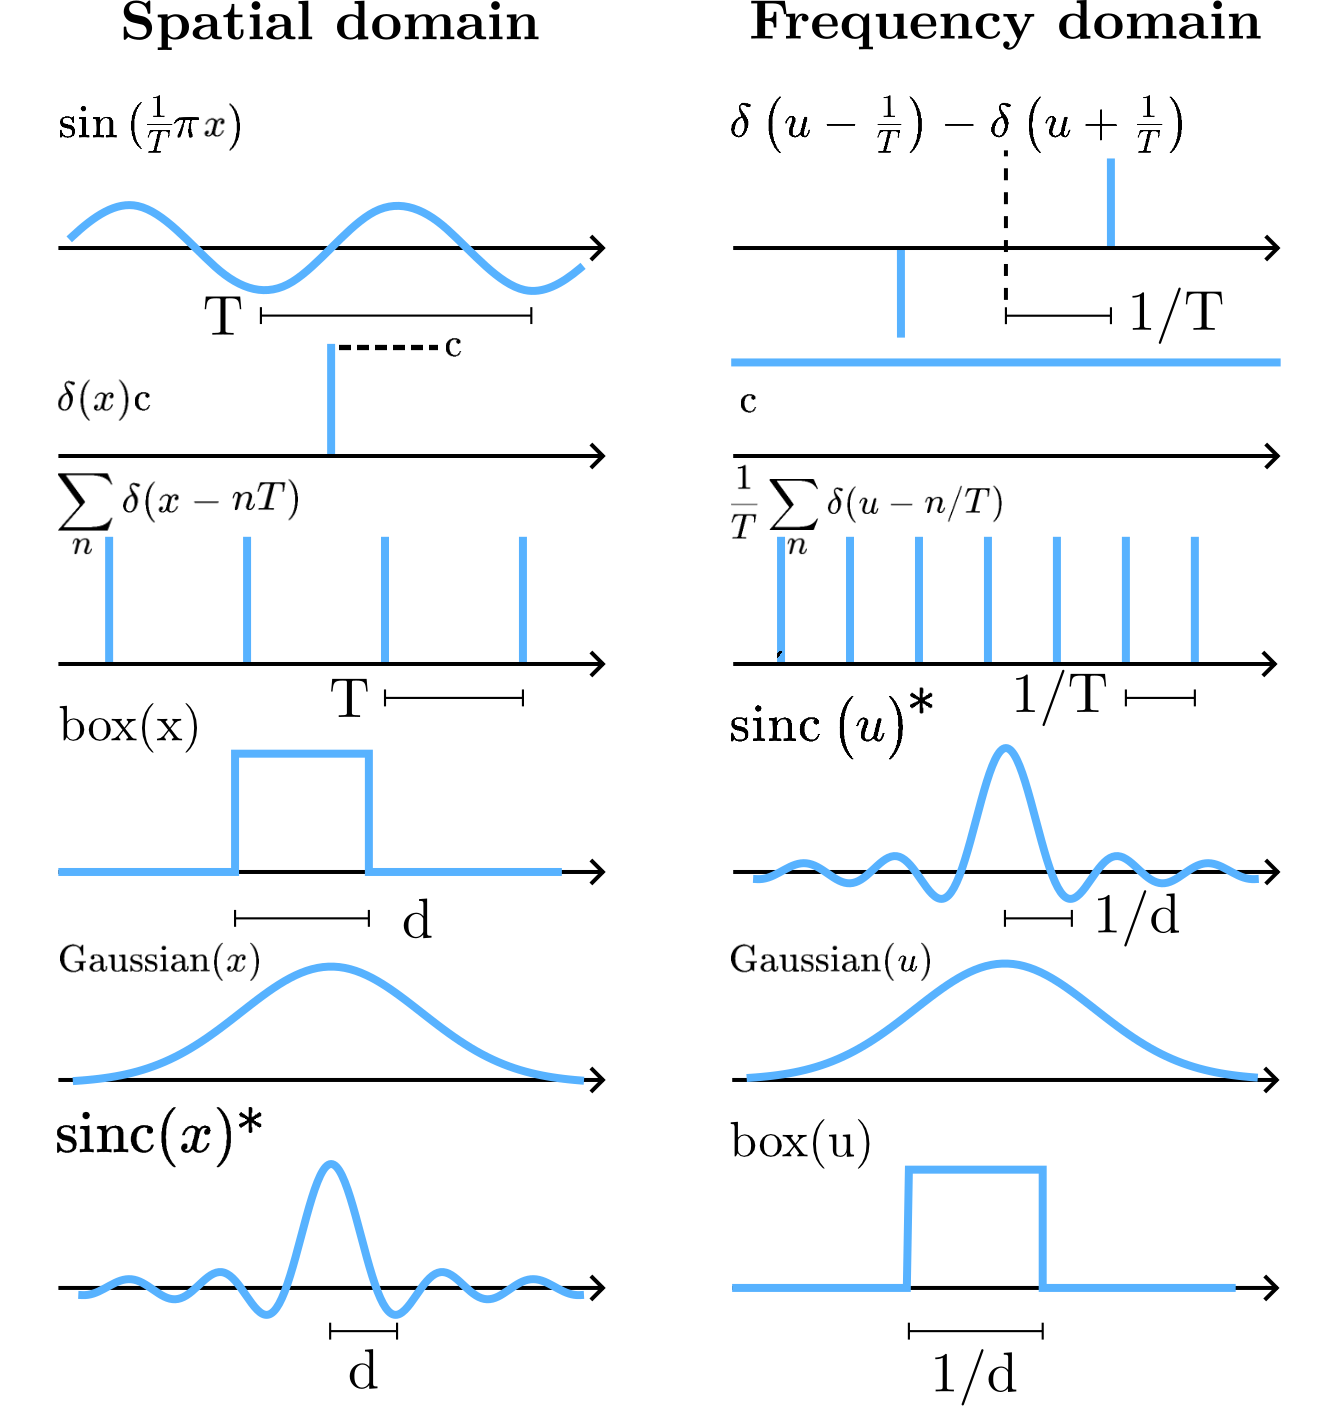
\includegraphics[scale=1]{../images/fourier-transforms.png} \\

\textbf{*} Holds if $\operatorname{sinc}(x)=\frac{\sin (\pi x)}{\pi x}$ (normalized), for $\frac{\sin (x)}{x}$ use $\operatorname{sinc}(\pi t) \rightarrow \operatorname{Box}(u)$ and $\operatorname{sinc}(\pi t) \rightarrow \operatorname{Box}(u)$\\
\textbf{Convolution Theorem}: Conv. in spatial domain = el. mult. in freq. domain and vice-versa: $\mathcal{F}[f * g]=F \circ G$ and $\mathcal{F}[f \cdot g]=F * G$. Can be used to efficiently compute convolution: $h * f=\mathcal{F}^{-1}[H \circ F]$, with $F=\mathcal{F}((\operatorname{Image}))$
\begin{itemize}[leftmargin=*]
\item \textbf{Low-pass (Smoothen)}: $H_{low,\sigma}= \mathcal{F}(G_{\sigma}(x,y))$
\item \textbf{High-pass (Sharpen)}: $H_{high, \sigma}= 1 - H_{low, \sigma}$
\item  \textbf{Band-pass}: $H_{band, [\sigma_1, \sigma_2]}= H_{low,\sigma_1} - H_{low,\sigma_2}$
\end{itemize}


\mysubsection{1.6 Unitary Transform}
\textbf{Linear Operations}: $O(\alpha x+\beta y)=\alpha O(x)+\beta O(y)$ $\alpha, \beta \in \mathbb{R}$. Alt. Matrix $\mathbf{O}$. For pictures $I\in \mathbb{R}^{M_1 \times M_2}$, with $N = M_1 \times M_2$ we have $c=\mathbf{O}f$, $c,f \in \mathbb{R}^{N}, \mathbf{O}^{N\times N}$\\
\textbf{Unitary Operations}: Lin. Op. with $\mathbf{O}^{-1}=\mathbf{O}^{H}$. Preserves Norm/Energy: $\|c\|^2=f^H A^H A f=\|f\|^2$\\
\textbf{Auto-Correlation}: $R_{\mathrm{ff}}=E\left[f_i \cdot f_i^H\right]=\frac{F \cdot F^H}{n}$. $R_{f f}(i, j)$ denotes how pixel $f_i$ correlates with pixel $f_j$. $R_{\mathrm{ff}}\in \mathbb{R}^{N}$, $R_{c c}=\mathbb{E}\left[c c^H\right]=\mathbb{E}\left[A f f^H A^H\right]=A R_{f f} A^H$\\

\textbf{Eigenmatrix}: $\Phi$ of autocorrelation matrix $R_{\mathrm{ff}}: \Phi$ is unitary, columns form set of eigenvectors of $R_{\mathrm{ff}}$: $R_{\mathrm{ff}} \Phi=\Phi \Lambda$ where $\Lambda$ is a diag. matrix of eigenvecs. $R_{\mathrm{ff}}$ is symmetric nonneg. definite, hence $\lambda_i \geq 0$, and normal: $R_{\mathrm{ff}}^H R_{\mathrm{ff}}=$ $R_{\mathrm{ff}} R_{\mathrm{ff}}^H$.\\

\textbf{Eigenspace Matching}: Find similar image $I_{c}$ to set of $n$ images $I_i$.${\arg \min_i } D_i=\left\|\mathrm{I}_i-\mathrm{I_c}\right\|$. Autocorr. all options expensive. Preselect with ${\arg \min_i } D_i=\left\|\mathrm{p}_i-\mathrm{p_c}\right\|$ where $p=\mathbf{E}^{T}\hat{I}$ (Eigenval. Dec.), $\hat{I}= I - \bar{I}$, $\bar{I}=\frac{1}{n}\sum^{n} I_i$. Same can be done with SVD.

\textbf{Eigenfaces}: Eigenspace Matching for faces, struggle with lighting differences. \\
\textbf{Fisherfaces}: Improvement of EF by maximizing be-tween-class scatter, minimzing within-class scatter. Solution given by Eigenval. Dec: $\mathbf{R_B W}=\mathbf{R_W W \Lambda}$. $\operatorname{rank}(\mathbf{R_W})=C$, where $C$ amount of different classification classes. Transf. to $C$-dim subspace by PCA  \\
\textbf{Find faces} on $I$ with dataset of faces ($d$): 1. PCA of $d$, 2. take patch $I$, 3. comp. reconstr. err. ($e$), 4. repeat for each patch, 5. find loc. with min. $e$.
\BCODE{Principal Component Analysis}{
\begin{enumerate}[leftmargin = *,noitemsep]
\item \textit{Normalize to remove brightness var.:} $x_i^{\prime}=\frac{x_i}{\left\|x_i\right\|}$ 
\item Center data by subtracting mean: $x_i^{\prime \prime}=x_i^{\prime}-\mu, \mu=$ $\frac{1}{N} \sum x_i^{\prime}$
\item Compute covar. mat.: $\Sigma=\frac{1}{N-1} \sum x_i^{\prime \prime} \cdot \left(x_i^{\prime \prime}\right)^T$ 
\item Compute eigendecomp. of $\Sigma$ by solving $\Sigma e=\lambda e$ with e.g. $\operatorname{SVD}\left(\Sigma=\mathbf{U} \Lambda \mathbf{U}^T\right)$

\item Define $U_k$ as first k eigenval. of $\Sigma, U_k=\left(\begin{array}{lll}u_1 & \ldots & u_k\end{array}\right)$ directions with largest variance centered at mean, perpendicular

\item $\operatorname{PCA}\left(x_i\right)=U_k^T\left(x_i-\mu\right)=U_k^T \cdot x_i^{\prime \prime}$

\end{enumerate}

To decompress, use $\mathrm{PCA}^{-1}\left(x_i\right)=U_k \cdot y_i+\mu$

}
\textbf{Applications}: Face detect. Data compr. Data vis.\\
\textbf{PCs}: $n=\# \operatorname{PCs}$,$m= \operatorname{dim} \text{samples}$, $o= \# \text{samples}$  :

\begin{itemize}[leftmargin = *,noitemsep]
\item $n\leq m$: Can't have more than $m$ $\perp$ vect. 
\item $n\leq o$: $\operatorname{rank}\Sigma \leq m$
\end{itemize}





\textbf{Storage Space}: $I\in \mathbb{R}^{a\times a}, I_{compr}\in \mathbb{R}^{K}$ tot. space: $a^2$ (mean) $+a^2K$ ($U_{k}$) $+nK$ (compr. Image)

\mysubsection{1.7 JPG \& JPEG}
\begin{enumerate}[leftmargin = *,noitemsep]
\item Convert RGB $\rightarrow$ YUV (Y luminance / brightness, UV color / chrominance). Humans more sensitive to color, compress colors with chroma subsampling (e.g. color of upper left pixel for $4 \times 4$ grid)

\item Split image into $8 \times 8$ blocks for each YUV component, apply 2D DCT to it. 64 values, top left $=$ low freq., bottom right $=$ high freq. DCT: variant of DFT, fast implementation, only real values

\item Compress using int. devision with weighted matrix (Quantization table), compress bottom-right. Zig-zag run length encoding followed by Huffman.
\end{enumerate}

High compression $(10-100 \mathrm{x})$ and 24 -bit colors possible, but artifacts / incorrect colors / aliasing. Edges are softened because sharp edges require high freq. JPEG2000 improves by using Haar transform globally, not just on $8 \times 8$ blocks, on successively downsampled image (image pyramid)

\textbf{Image pyramids}: iter. applied approx. filter / downsampler. Gaussian pyramid, Laplacian is difference between 2 levels in Gaussian pyramid.\\
\textbf{Haar transform}: Scaling capture info. at diff. freq.,Translate captured info. at diff. loc. Can be repr. by filter+downsample. Poor energy compaction.



\mysubsection{1.8 Optical Flow}
Apparent motion of brightness patterns. We set $u=\frac{\mathrm{d} x}{\mathrm{~d} t}$,$
v=\frac{\mathrm{d} y}{\mathrm{~d} t}, I_x=\frac{\partial I}{\partial x}, I_y=\frac{\partial I}{\partial y}, I_t=\frac{\partial I}{\partial t}$


\textbf{Brightness constancy}: $
I(x, y, t)=I\left(x+\frac{\mathrm{d} x}{\mathrm{~d} t} \partial t, y+\frac{\mathrm{d} y}{\mathrm{~d} t} \partial t, t+\partial t\right) \overset{\underset{\mathrm{taylor}}{}}{\approx} I(x, y, t)+\frac{\partial I}{\partial x}\left(\frac{d x}{d t} \delta t\right)+\frac{\partial I}{\partial y}\left(\frac{d y}{d t} \delta t\right)+\frac{\partial I}{\partial t}(\delta t)$


\textbf{Optical flow constraint}:$
\frac{\mathrm{d} I}{\mathrm{~d} t}=\frac{\partial I}{\partial x} \frac{\mathrm{~d} x}{\mathrm{~d} t}+\frac{\partial I}{\partial y} \frac{\mathrm{~d} y}{\mathrm{~d} t}+\frac{\partial I}{\partial t}=0$
\textbf{Aperture problem}: 2 unknowns for every pixel $(u, v)$ but only one equation $\Rightarrow \infty$ solutions (underdetermined SLE), opt. flow defines a line in $(u, v)$ space, compute normal flow. Need additional constraints to solve.
\BCODE{Horn \& Schunck Algorithm}{
\textbf{Assumption}: values $u(x, y), v(x, y)$ are smooth and change slowly with $x, y$.\\ Minimize $e_s+\lambda e_c$ for $\lambda>0$ where
$
\begin{aligned}
& e_s=\iint\left(\left(u_x^2+x_y^2\right)+\left(v_x^2+v_y^2\right)\right) \mathrm{d} x \mathrm{~d} y \text { (smooth.) } \\
& e_c=\iint\left(I_x u+I_y v+I_t\right)^2 \mathrm{~d} x \mathrm{~d} y \text { (bright. const.) }
\end{aligned}
$

Coupled PDEs solved using iter. methods and finite diffs: $\frac{\partial u}{\partial t}=\Delta u-\lambda\left(I_x u+I_y v+I_t\right) I_x$ and $\frac{\partial v}{\partial t}=\Delta v-$ $\lambda\left(I_x u+I_y v+I_t\right) I_y$. Has errors at boundaries / information spreads from corner-type patterns.
}

\BCODE{Lucas-Kanade }{
Assumption: neighb. in $N \times M$ patch $\Omega$ have same motion $(u v)^{\top}$, small mov., bright. const.
$E=\sum_{x, y \in \Omega}\left(I_x(x, y) u+I_y(x, y) v+I_t(x, y)\right)^2$
$M U=\left(\begin{array}{cc}\sum I_x^2 & \sum I_x I_y \\ \sum I_x I_y & \sum I_y^2\end{array}\right)\binom{u}{v}=-\binom{\sum I_x I_t}{\sum I_y I_t}\left(\sum\right.$ over patch $\left.\Omega\right)$
First compute $I_x, I_y, I_z$. Let $M=\sum(\nabla I)(\nabla I)^T$ and $b=$ $\left(-\sum I_x I_t-\sum I_y I_t\right)$ Then at each pixel, compute $U$ by solving $M U=b$ by using least squares $U=M^{-1} b=$ $\left(M^T M\right)^{-1} M^T b$. If $M$ singular / fails if all gradient vec. in same dir (along edge, smooth regions). Works with corners, textures.

}



\textbf{Iterative refinement}:
Estimate OF with Lucas-Kanade. Warp image using estimate OF. Estimate OF using warped image. Refine by repeating and add up all estimates. \textbf{Gradient method} fails when intensity structure within window is poor, displacement large, inconstant light, sol: \textbf{CtFE}\\
\textbf{Coarse-to-fine Estimation}:
Create levels by gradual subsampling. Start at coarsest level, estimate OF, iterate and add until reached finest level. Still fails if large lighting changes happen.\\
\textbf{Affine Motion}: Each pixel provides 1 lin. constr., 6 global unknowns. Solve LSE. From bright. const. eq.:$I_x\left(a_1+a_2 x+a_3 y\right)+I_y\left(a_4+a_5 x+a_6 y\right)+I_t \approx 0$



\textbf{SSD tracking}: Large displacements, extract template around pixel, match within search area, use correlation, choose best match.\\
\textbf{Bayesian Optical flow}: Some low-level human motion illusions can be explained by adding an uncertainty model to LK. E.g. bright. const. with noise.

\mysubsection{1.9 Video Compression}

Visual perception $<24 \mathrm{~Hz}$. Flicker $>60 \mathrm{~Hz}$ in periphery.\\
\textbf{Bloch's law}: If stimulus duration $\leq 100 \mathrm{~ms}$, duration and brightness exchangeable. If brightness is halved, double duration. This enforces $>10 \mathrm{~Hz}$ for videos.\\
\textbf{Interlaced video format}: 2 temporally shifted half images (in bands) increases frequency, reduces spatial resolution. Full image repr. is progressive.


\BCODE{Video Compression w/ Temporal Redundancy}{

Predict current frame based on previously coded frames. Introducing 3 types of coded frames:
\begin{enumerate}[leftmargin = *,noitemsep]
\item I-frame: Intra-coded frame, coded independently
\item P-frame: Predictively-coded based on previously coded frames (e.g. motion vec. + changes)
\item B-frame: Bi-directionally predicted frame, based on both previous and future frames.
\end{enumerate}

Inefficient for many scene changes or high motion.
}


\textbf{Motion-compensated prediction}: partition video into moving objects - generally pretty difficult. \\
\textbf{Block-Matching Motion Est.}: partition each frame into blocks, describe motion of block / find best matching block in reference frame. No obj. det., good perf. Can be sped up with 3 step log search, and improve precision with half-pixel motions. We encode the residual error (with JPG). Motion vector field (set of motion vec. for each block in frame) is easy to encode, fast, simple, periodic, practical.\\

\textbf{MPEG Group of Pictures (GOP)}: Starts with I-frame, ends with B- ("open") or P-frame ("closed")


\mysubsection{1.10 CNN \& Radon Transform}

Given input $x$, learning target $y$, loss function $\mathcal{L}$ compute kernel weights $\theta$ using prediction $f(x, \theta)$ : $\arg \min _\theta \mathcal{L}(y, f(x, \theta))$. Linear classifier $f(x, \theta)=$ $W x+b$ where $\theta=\{W, b\}$. Use activation func. $\phi$ (sigmoid, ReLU, tanh, ...) to introduce non-linearity. Use gradient descent and back propagation (recursive appl. of chain rule to compute gradients) to find $\theta$. Transformers, GANs, stable diffusion etc enable modern VC breakthroughs.

\textbf{Classification}: $f\left(x_1, \theta\right)$ as score, take class with larger score. With $y_i \in \mathbb{N}, s_i=f\left(x_i, \theta\right)$, we get loss function: $\mathcal{L}(y, f(x, \theta))=-\sum_{i=1}^N \log \left(\frac{\exp \left(s_{i, y_i}\right)}{\sum_j \exp \left(s_{i, j}\right)}\right)$\\
\textbf{Regression}: $f\left(x_1, \theta\right)$ as value, can be used for classification by comparing value. With $y_i \in \mathbb{R}^n, s_i=f\left(x_i, \theta\right)$, we get: $\mathcal{L}(y, f(x, \theta))=\sum_{i=1}^N\left\|y_i-s_i\right\|^2$


\BDEF{Radon transform }{Given object with unknown density $f(x, y)$, find $f$ by sending rays from all dirs through object and measure absorption on the other. side. Assume parallel beams for given angle and no spreading of beam. X-Ray along line $L$ at distance $s$ has intensity $I(s)$, travelling $\partial s$ reduces intens. by $\partial I$. reduction depends on intens. and optical density $u(s)$ : $\frac{\partial I}{I(s)}=-u(s) \partial s$. Radon transform of $f(x, y): R f(L)=$ $\int_L f(x)|\mathrm{d} x|$. With $(x, y)=(\rho \cos \theta-s \sin \theta, \rho \sin \theta+$ $s \cos \theta)$ we get: $R(\rho, \theta)=\int u(x, y) \mathrm{d} s$. We now want to find $u(x, y)$ given $R(\rho, \theta)$.
}

The continuous case of a radon transform of a line is:

$$
R(\rho, \theta)=\int_{-\infty}^{\infty} \int_{-\infty}^{\infty} u(x, y) \delta(\rho-x \cos \theta-y \sin \theta) \partial x \partial y
$$
\textbf{Properties of RT}: Linear, shifting input shifts the RT, rotating input rotates RT, RT of 2 D convolution is 1D convolution of RT with respect to $\rho\left(R\left(f *_{2 \mathrm{D}} g\right)=\right.$ $R(f) *_{1 \mathrm{D}} R(g)$, RHS with fixed $\left.\theta\right)$


\begin{center}
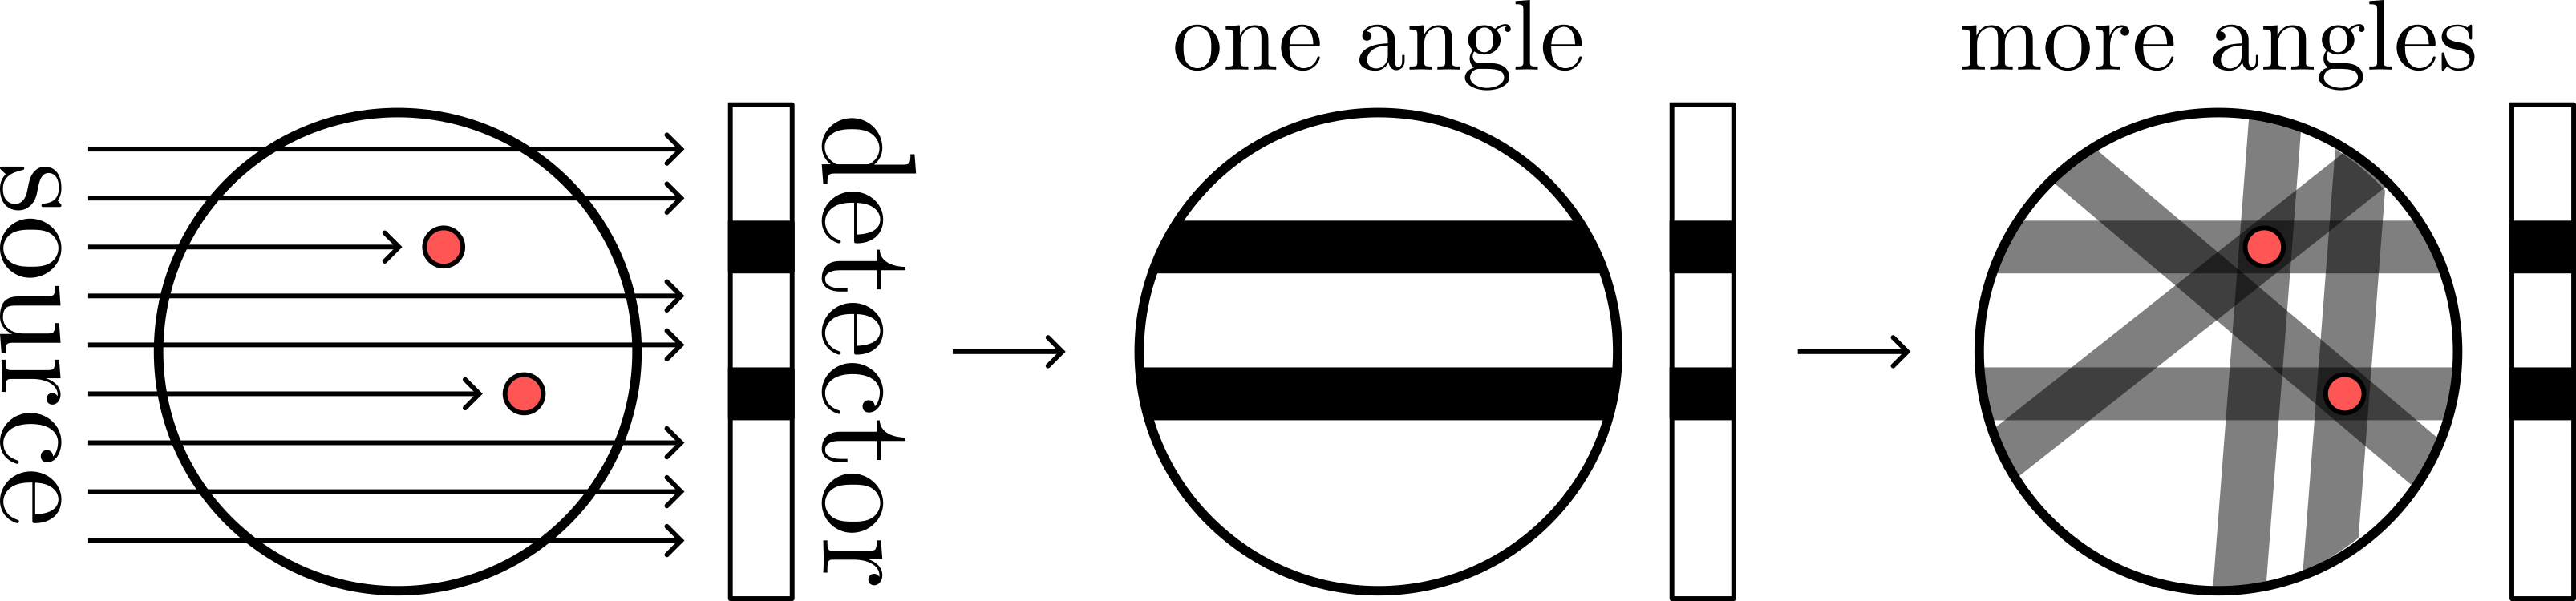
\includegraphics[scale=0.3]{../images/radon-back-projection.png} 

\end{center}
\BCODE{Back Projection}{
Given RT, find $u(x, y)$
Fourier slice thm (apply with all proj. angles $\theta$ ):
\begin{enumerate}[leftmargin = *,noitemsep]
\item \textbf{Measure attenuation data}: Measured along lines parameterized by $\rho$ = perp. distance from origin and $\theta$ = the angle of proj.
$$
R(\rho, \theta)=\int_{L(\rho, \theta)} f(x, y) d s
$$
\item \textbf{1D FT of projection data}: Convert to freq. domain. $\omega$ represents the frequency in the radial direction for the projection at angle $\theta$.
$$
\hat{R}(\omega, \theta)=\mathcal{F}_{1D}\{R(\rho, \theta)\}=\int_{-\infty}^{\infty} R(\rho, \theta) e^{-i \omega \rho} d \rho
$$
\item \textbf{2D inverse FT and sum with previous image (backpropagate)}: $$
u(x, y)=\mathcal{F}_{2D}^{-1}\left\{\sum_\theta \hat{R}(\omega, \theta)\right\}
$$
\end{enumerate}
Requires precise attn. meas., sensitive to noise, unstable, hear to implem., blurring in final image. Add high-pass filter in Fourier domain after 2nd step.
}